%! TEX program = xelatex
\documentclass[11pt,aspectratio=169]{beamer}
\usepackage{amsthm,amsmath,amssymb,braket,appendixnumberbeamer,pifont,fontspec,multicol,unicode-math,xcolor}
\usepackage{tcolorbox}
\definecolor{lightgray}{RGB}{226,226,226}
\newcommand{\eqbox}[1]{
\centering
\begin{tcolorbox}[width=\textwidth,
                  boxsep=0pt,
                  left=0pt,
                  right=0pt,
                  top=5pt,
                  bottom=10pt,
                  arc=0pt,
                  boxrule=0pt,toprule=0pt,
                  colback=lightgray,
		  frame empty
                  ]%%
\[{#1}\]
\end{tcolorbox}
}

\usepackage[absolute,overlay]{textpos}
\usetheme[numbering=none]{focus}

\setbeamerfont{alerted text}{series=\bfseries}

\usepackage[backend=bibtex,url=false,doi=false,maxcitenames=1, style=authoryear]{biblatex}

\newcommand{\nitem}{\item}
\bibliography{bib}

\graphicspath{{./figures/}}

\title{Frustrating the Kondo Effect through Charge Fluctuations: from the Auxiliary Model to the Bulk}

\author{Abhirup Mukherjee}

\date{\today}

\institute{\it Emergent Phenomena in Quantum Matter\\ IISER Kolkata, Mohanpur
}

\begin{document}

\centering

\begin{frame}
\maketitle
\end{frame}

\section{Outline of the Discussion}

\begin{frame}{Outline of the Discussion}
\begin{itemize}
	\item Some {\bf preliminaries}: Hubbard model, DMFT, and the Anderson impurity model\vspace{\fill}
	\item What, then, are the {\bf questions}?\vspace{\fill}
	\item Explaining the Mott MIT: the {\bf extended} Anderson impurity model\vspace{\fill}
	\item Some more {\bf questions}!\vspace{\fill}
	\item {\bf Tiling} with the extended Anderson impurity model\vspace{\fill}
\end{itemize}

\end{frame}

\section{The Hubbard model}

\begin{frame}{The Hubbard model: What and Why}

\includegraphics[width=0.5\textwidth]{Hubbard.pdf}

\eqbox{
H_\text{hub} = -t\sum_{i,j}\left(c^\dagger_{i\sigma}c_{j\sigma} + \text{h.c.}\right) + U\sum_i n_{i \uparrow}n_{i \downarrow} - \mu N
}

\(U/t=0 \longrightarrow\) free electron model \hspace{\fill} \(U/t=\infty\longrightarrow\) array of free spins\\[10pt]
\alert{Is there a transition at finite \(U/t\)?}
\end{frame}

\begin{frame}{The Hubbard model: What and Why}

\begin{minipage}{0.59\textwidth}
	\alert{Believed to describe the physics of the cuprates}\\[10pt]

\begin{itemize}
	\item inert spacer layers render the material quasi-2D
	\item physics happens in the Cu-O planes
	\item 3d-electrons from copper hybridise with the oxygen p-orbitals
\end{itemize}
\end{minipage}
\begin{minipage}{0.4\textwidth}
	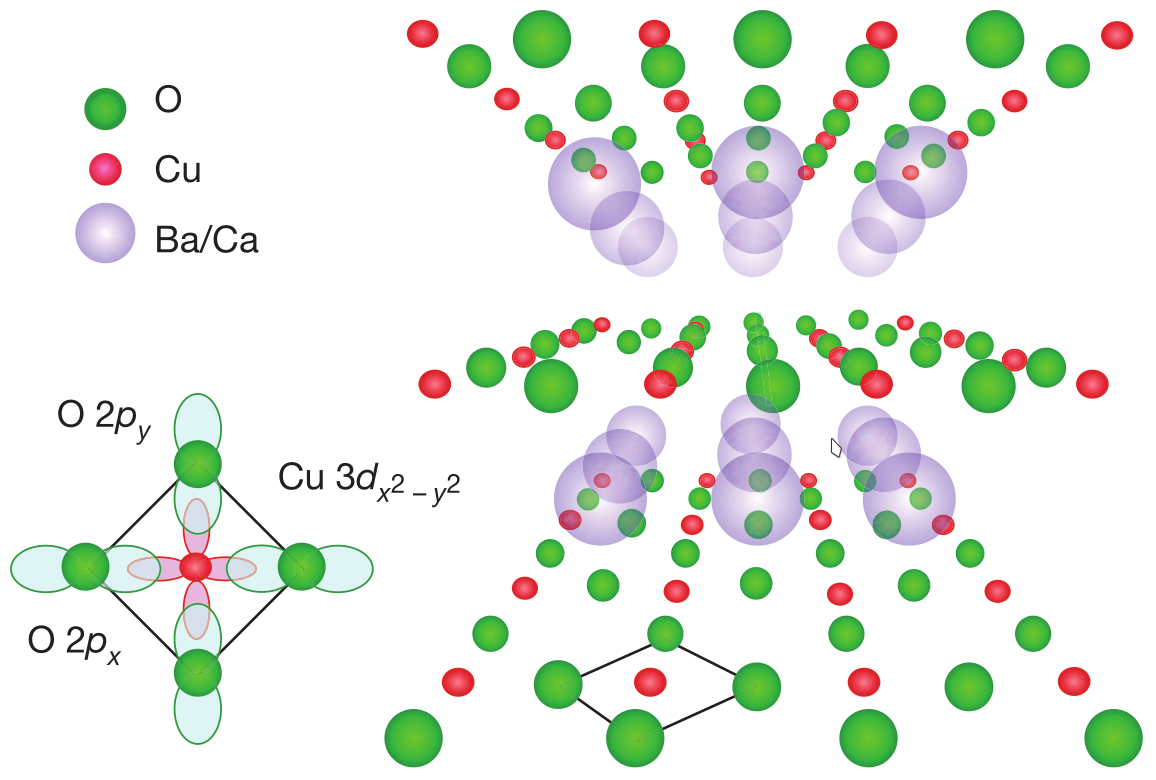
\includegraphics[width=\textwidth]{cuprates.png}
\end{minipage}

\vspace*{\fill}

Might also describe superconducting Nickelate (replace Cu with Ni) and organic charge transfer salts

\footnotetext[0]{Keimer et al., Nature (2015); ~ Souza1 and Pouget, JPCM (2013);~ Qin et al., Annu. Rev. Condens. Matter Phys (2022);~Kitatani at al., NPR Quantum Mater (2020)}

\end{frame}

\begin{frame}{The Hubbard model in infinite dimensions}

\eqbox{
	H_\text{hub} = \underbrace{-t\sum_{\left<i,j\right>}\left(c^\dagger_{i\sigma}c_{j\sigma} + \text{h.c.}\right)}_{N\times z \text{ terms}} + \underbrace{U\sum_i n_{i \uparrow}n_{i \downarrow} - \mu N}_{N \text{ terms}}
}
	In order to retain competition between \(t\) and \(U\): 
	\[t \to t/\sqrt{z}\]
	\[\text{Enormously simplifies calculations:} \quad \Sigma(\vec k,\omega) = \sum_{\vec r}e^{i \vec{k}\cdot\vec{r}}\Sigma(\vec r, \omega), \quad \Sigma(\vec r, \omega) \sim z^{-r/2}\]
	\[\Sigma(\vec k,\omega) = \Sigma_\text{local}(\omega) \quad:\quad\text{\alert{lattice self-energy becomes independent of momentum}}\]
	\[\text{How to calculate this local self-energy? DMFT!}\]

	\footnote{Miiller-Hartmann, Z. Phys. B-Condensed Matter (1989); Metzner and Vollhardt, PRL (1989); Georges et al, RMP (1996)}
\end{frame}


\section{Dynamical mean-field theory}

\begin{frame}{How does classical mean-field theory work?}
\begin{itemize}[<+->]
	\item Replace fluctuations by an \alert{effective mean field} $h(y)$, where \(y\) is some order parameter.
		\only<1>{\color{brown}\[J \sum_i S_i^z S_{i+1}^z \to h \sum_i S_i^z, h=\beta J m\]}\\[10pt]
\item Construct a \alert{self-consistency equation} for the simplified model, typically of the form: $y = f(h)$.
	\only<2>{\color{brown}\[m = \tanh(h)\]}\\[10pt]
\item By starting with some \alert{guess value \(h_\text{guess}\)} for the mean-field, calculate the order parameter \(y_\text{guess}\) corresponding to the guess field.
	\only<3>{\color{brown}\[h=0.01\implies m=0.02 (say)\]}\\[10pt]
\item From the consistency equation, the order parameter gives the next value of the field: \(h = f^{-1}_\text{next}(y_\text{guess})\), leading to an \alert{updated mean-field Hamiltonian}.
	\only<4>{\color{brown}\[h=0.01\implies m=0.02 \implies h_\text{next} = \arctan(0.02)\]}\\[10pt]
\item \alert{Keep solving} this updated Hamiltonian until the order parameter resulting from subsequent iterations does not change.
	\only<5>{\color{brown}\[h=0.059\implies h_\text{next} = \arctan(0.0591) \implies h_\text{next} = \arctan(0.0589) \]}
\end{itemize}
	
\end{frame}
\begin{frame}{How does dynamical mean-field theory work?}

\begin{itemize}[<+->]
	\item Replace fluctuations by an \alert{effective mean field} $h(y)$, where \(y\) is some order parameter.

		\only<1>{\color{brown}\[\Sigma(\vec k,\omega) \to \Sigma_\text{loc}(\omega)\]}

	\item Construct a \alert{self-consistency equation} for the simplified model, typically of the form: $y = f(h)$.
		\only<2>{\color{brown}
			\[G_\text{loc} = 1/\left(\omega - t^2 G_\text{loc} - \Sigma_\text{loc}\right) \]
			\centering
		The RHS is the impurity Greens function of an \\
		\alert{Anderson impurity model} with bath described by \(G_\text{loc}\)!
	}

	\item By starting with some \alert{guess value \(h_\text{guess}\)} for the mean-field, calculate the order parameter \(y_\text{guess}\) corresponding to the guess field.

	\only<3>{\color{brown}\centering
		Create SIAM with Hubbard \(U\) and trial \(G_\text{loc}\)\\
		as the bath Greens function. Solve SIAM to obtain \(\Sigma_\text{loc}\)
	}

	\item From the consistency equation, the order parameter gives the next value of the field: \(h = f^{-1}_\text{next}(y_\text{guess})\), leading to an \alert{updated mean-field Hamiltonian}.

	\only<4>{\color{brown}\centering
		From \(G_\text{loc}\) and \(\Sigma_\text{loc}\), calculate the impurity Greens function, using
		\[G_\text{imp} = 1/\left(\omega - t^2 G_\text{loc} - \Sigma_\text{loc}\right)\]
		By the self-consistency equation, this is also \\
		the bath Greens function for next iteration.
	}

	\item \alert{Keep solving} this updated Hamiltonian until the order parameter resulting from subsequent iterations does not change.
	\only<5>{\color{brown}
		\[\text{The problem then reduces to finding a SIAM with }G_\text{imp} = G_\text{bath}.\]
		\[\text{This is done iteratively, through a ``self-consistency loop".}\]}
\end{itemize}

\end{frame}

\begin{frame}{DMFT Results on the Bethe lattice in \(d=\infty\), at \(1/2-\)filling}
\[\text{Local spectral function \alert{acquires a gap} at a critical value of \(\frac{U}{D} (\sim 3)\)}\]
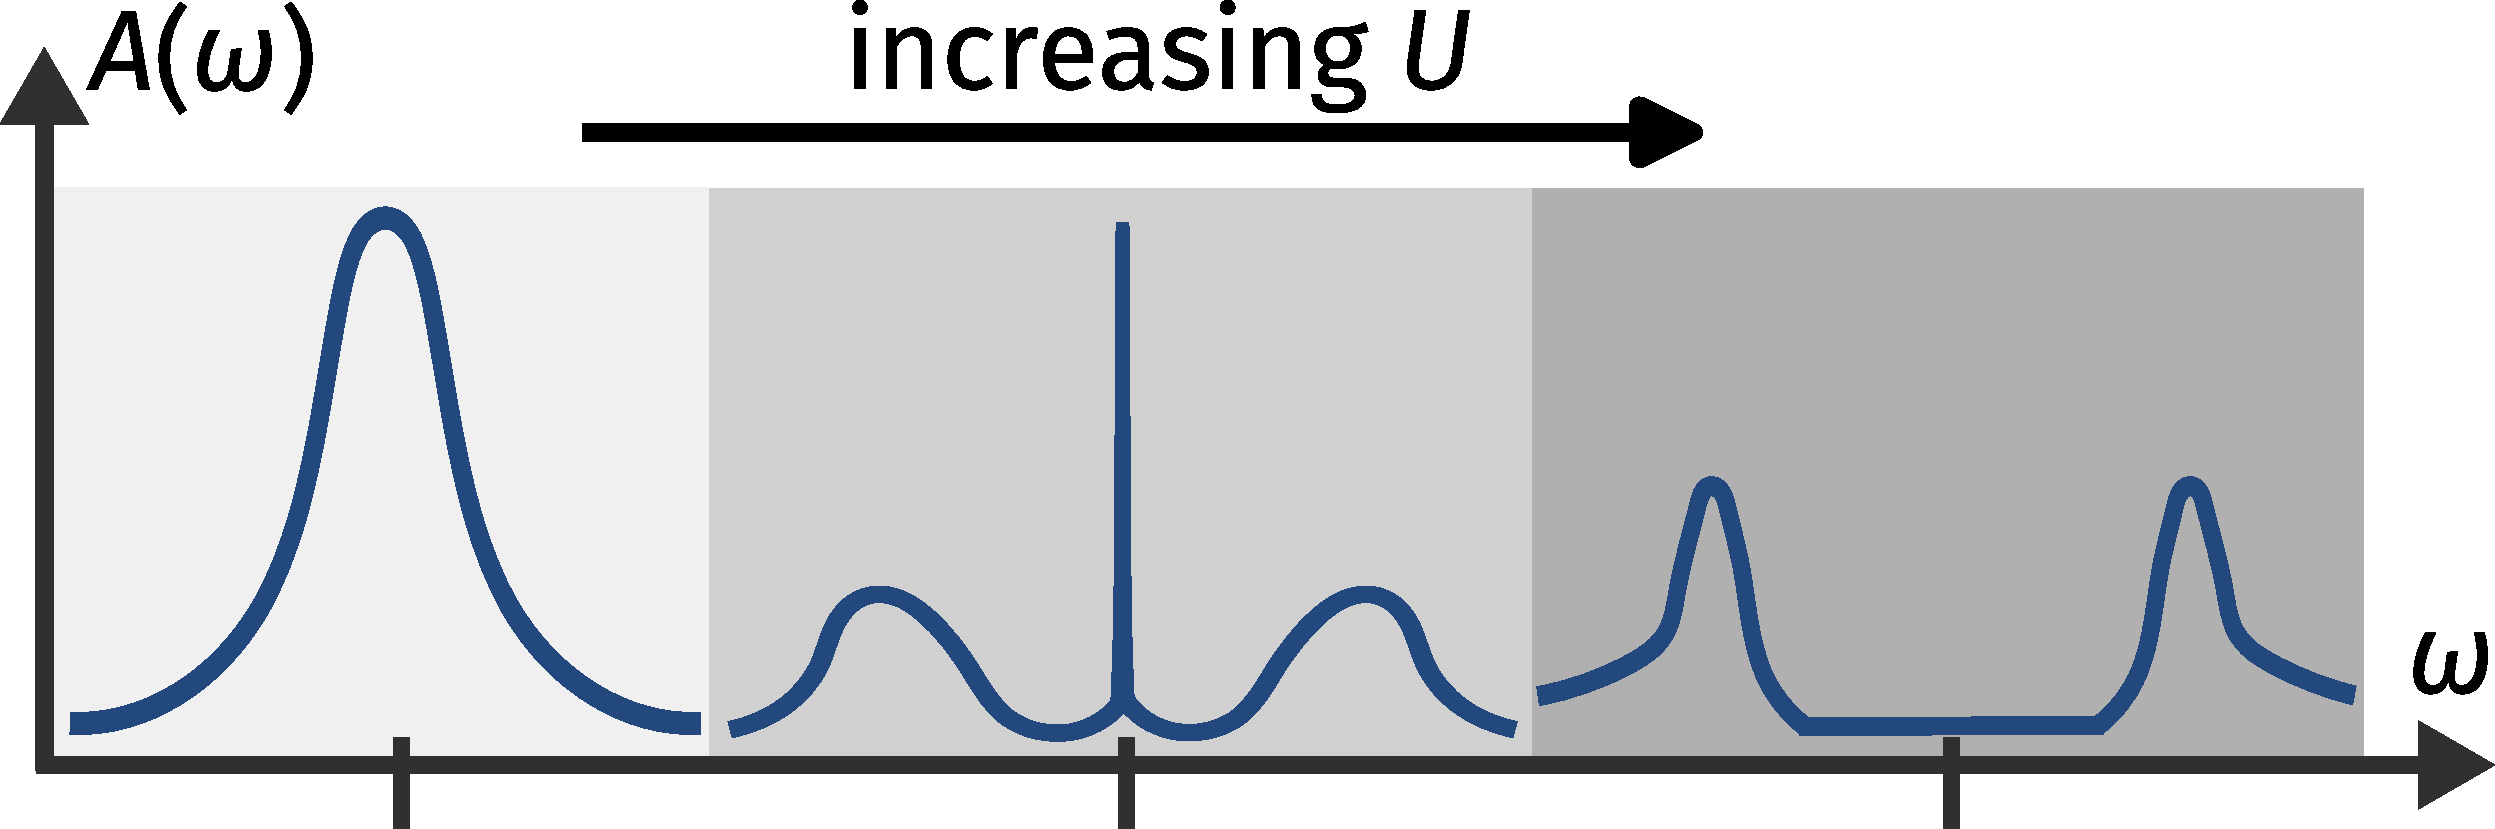
\includegraphics[width=0.5\textwidth]{dmft-sf.pdf}
\[\text{Constitutes a zero temperature \alert{Mott metal-insulator transition}}\]
\[\text{Good metal with broad peak}\Rightarrow\text{"Bad" metal with sharp peak}\Rightarrow\text{Mott insulator}\]
\end{frame}

\begin{frame}{DMFT Results on the Bethe lattice in \(d=\infty\), at \(1/2-\)filling}
\[\text{Transition is \alert{not bi-continuous}, scales do not vanish simultaneously on both sides}\]
\[\text{\(T=0\) second order point replaced by a first order line at finite temperatures}\]
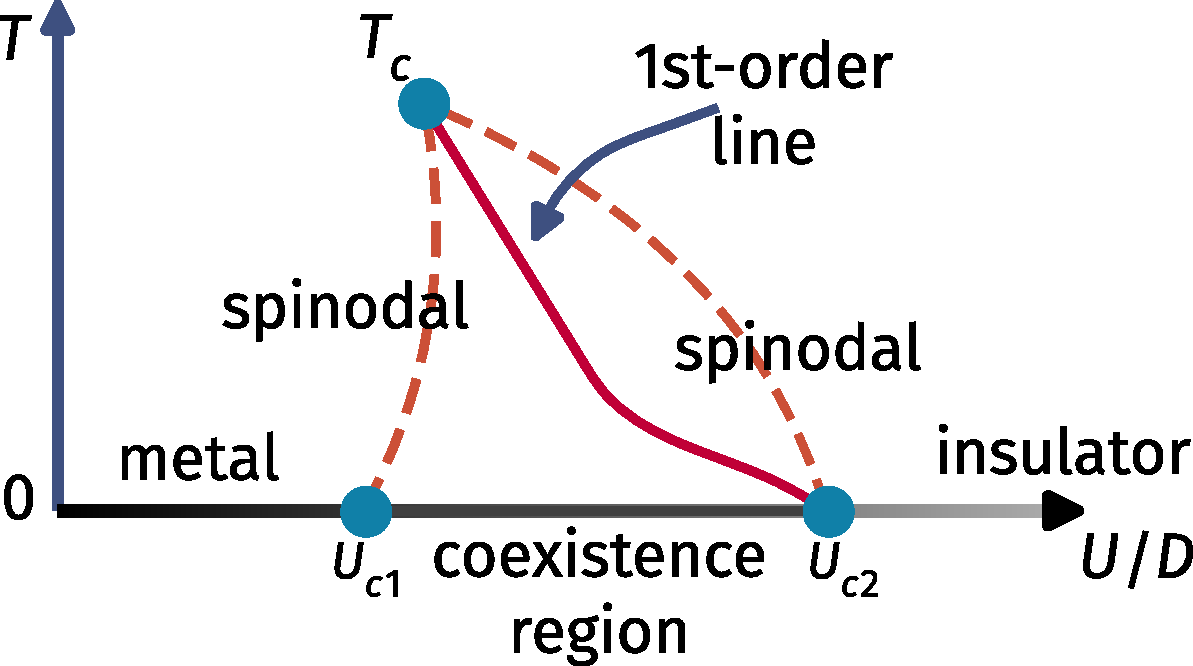
\includegraphics[width=0.5\textwidth]{coexistence-dmft.pdf}
\[\text{Leads to a \alert{metal-insulator coexistence region}, with a finite gap as well as central peak}\]
\end{frame}

\section{Physics of the Anderson impurity model}

\begin{frame}{Physics of the Anderson impurity model}
	\only<1>{Localised \(d-\) or \(f-\)electron hybridising with conduction bath}
	\only<1-3>{
	\eqbox{
	H_\text{SIAM} = \sum_{k}\epsilon_k n_{k\sigma} + \epsilon_d n_{d\sigma} + U n_{d \uparrow} n_{d \downarrow} + \sum_k \left[V(k)c^\dagger_{k\sigma}c_{d\sigma} + \text{h.c.}\right]
}
}
\only<1>{
	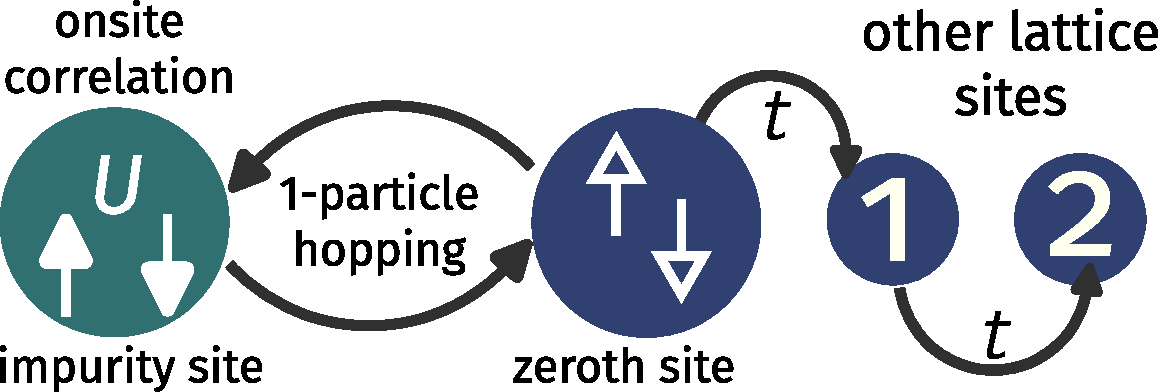
\includegraphics[width=0.5\textwidth]{siam_schematic.pdf}
}
\only<2>{
	\centering
	\[V/U > 0\]
	impurity strongly coupled to bath
	\[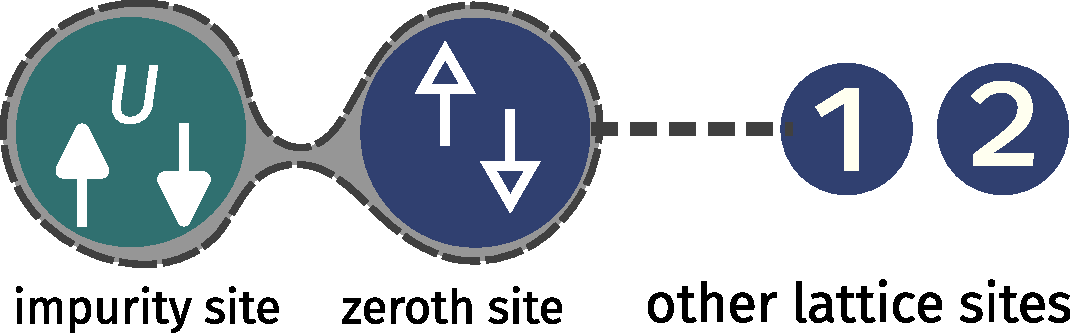
\includegraphics[width=0.5\textwidth]{siam_metallic.pdf}\]
	Gapless excitations are supported; spectral function \alert{has central peak}
}
\only<3>{
	\[V/U \to 0\]
	crossover to decoupled local moment
	\[
\includegraphics[width=0.4\textwidth]{siam_locmom.pdf}\]
	\[\text{spectral function acquires gap only at \(U/V = \infty\)}\]
	\alert{No phase transition} as \(U\) is tuned!
}
\only<4>{
	\begin{itemize}
		\item The standard \(1/2-\)filled SIAM has no local moment phase!
		\item \alert{Cannot explain} the Mott MIT of DMFT
		\item Self-consistency must be inserting additional physics.
	\end{itemize}
}


\end{frame}

\section{The Questions}

\begin{frame}{The Questions}
	\begin{itemize}[<+->]
		\item Is there a \alert{minimal but effective quantum impurity model} that describes the Mott MIT of the $1/2$-filled Hubbard model on the Bethe lattice in \(d=\infty\)?\vspace{20pt}
		\item What are the \alert{fluctuations that destroy the metal} and lead to the insulating phase? Can we obtain a universal theory for these competing tendencies?\vspace{20pt}
		\item Can such an impurity model explain the \alert{presence of two solutions} in the coexistence region? What about the spinodals and the first order line?\vspace{20pt}
		\item What is the origin of the \alert{quantum critical fluctuations} observed recently above the finite temperature second-order critical point?\vspace{20pt}
		\item What is the theory for the infrared gapless excitations \alert{precisely at the MIT}?
\end{itemize}
\end{frame}

\begin{frame}
\hspace*{-0.05\textwidth}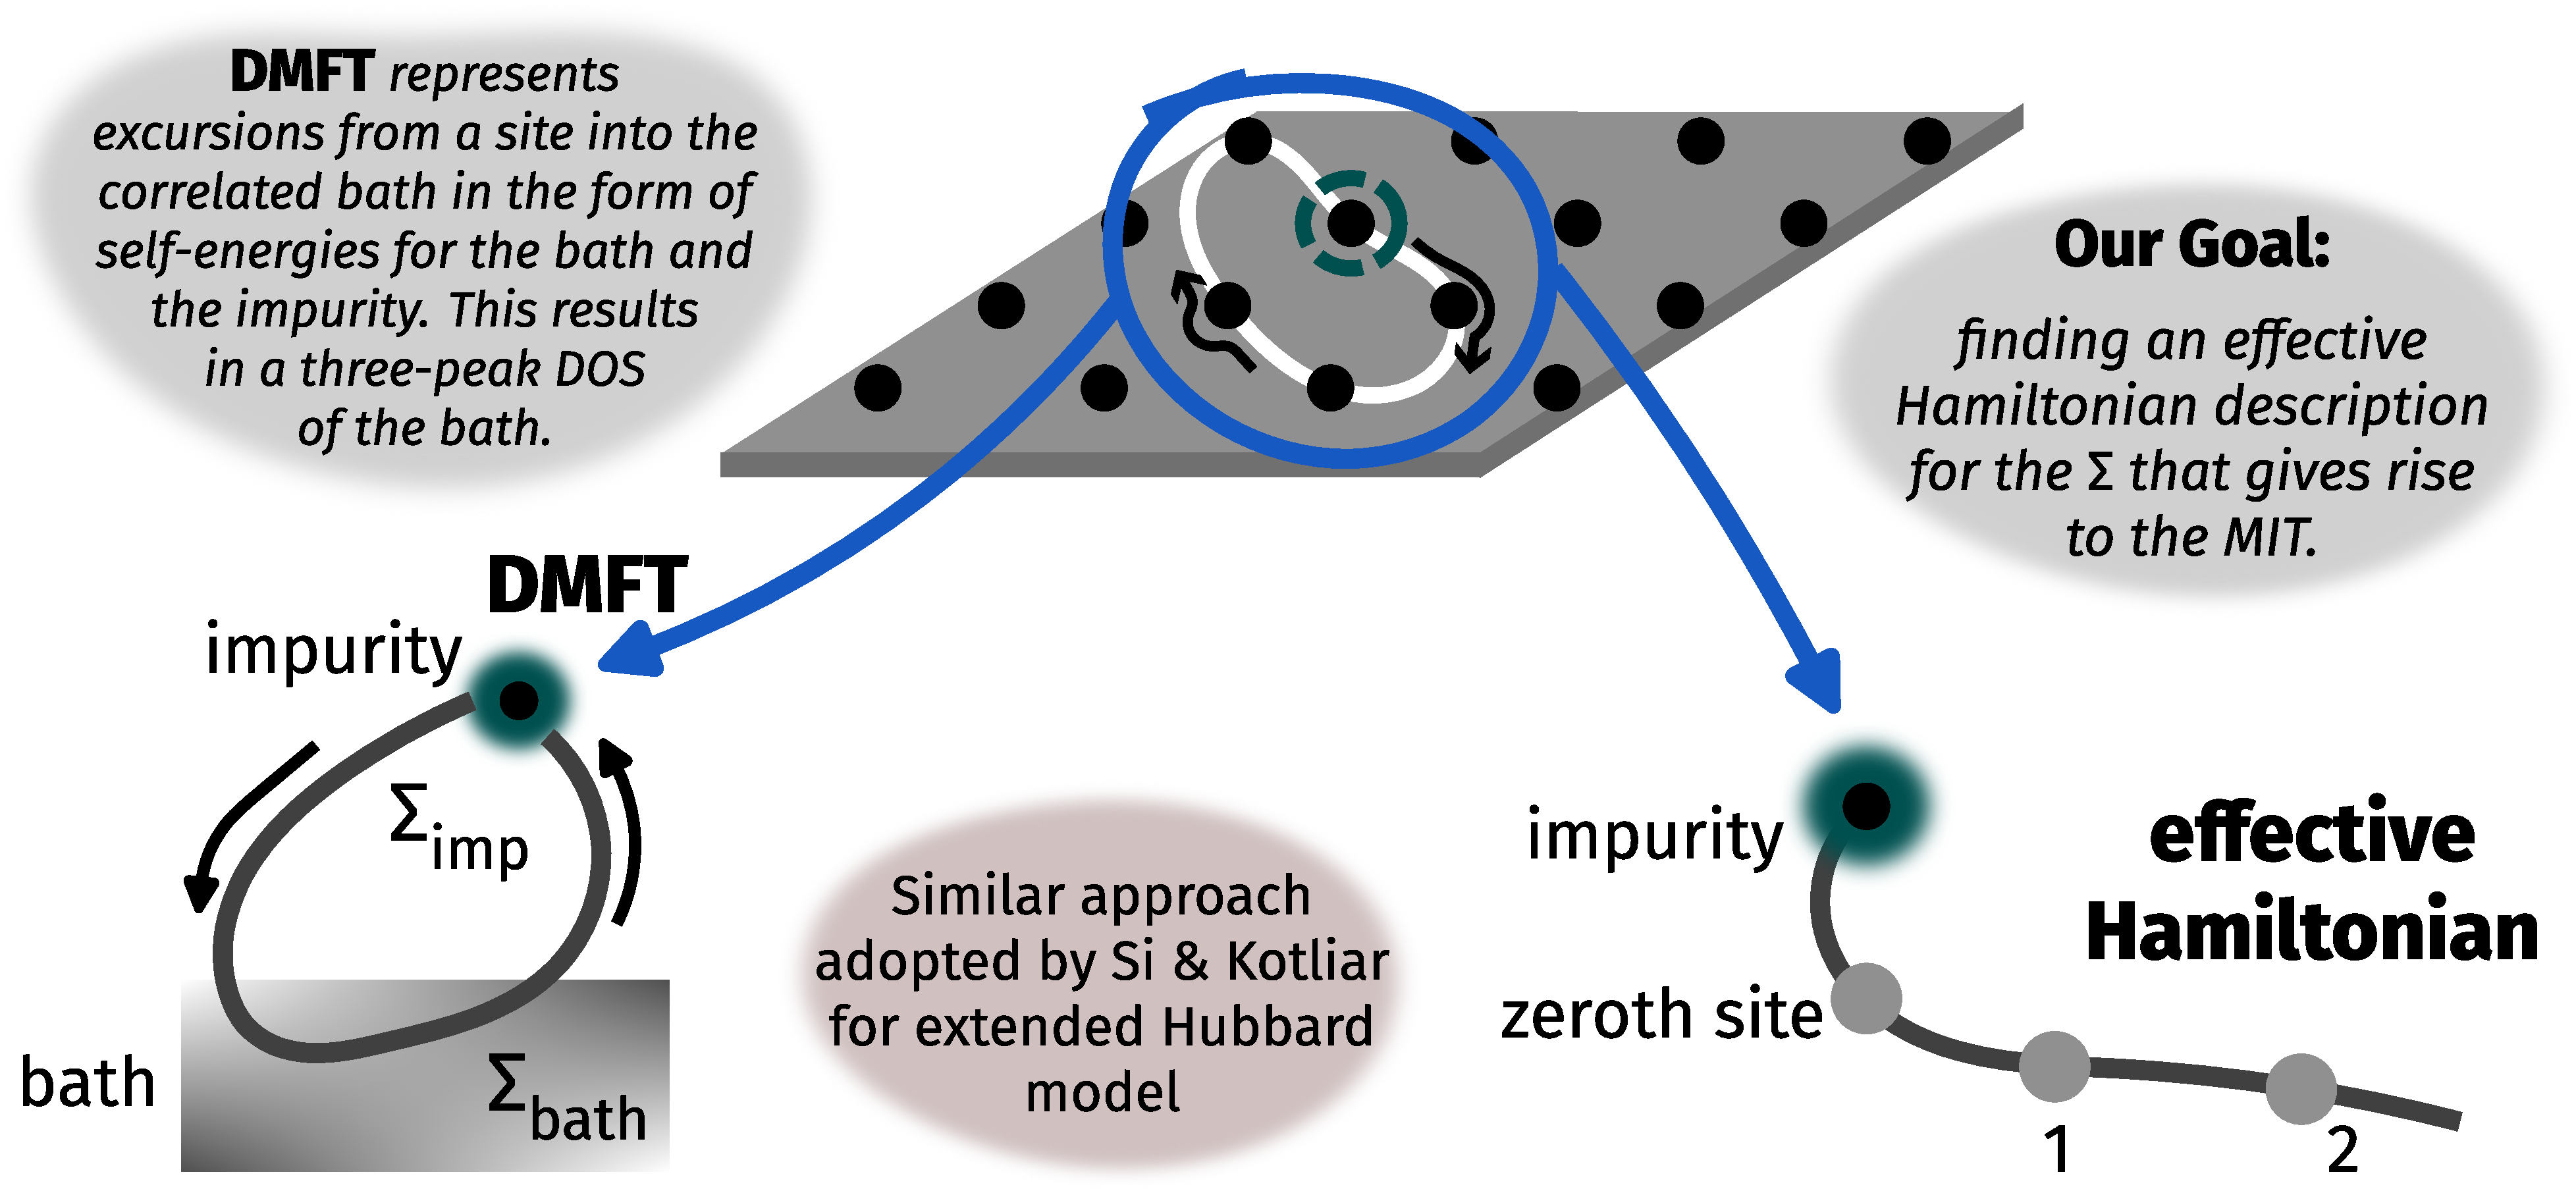
\includegraphics[width=1.1\textwidth]{contrast2.pdf}
\end{frame}

\section{Extending the Anderson impurity model}

\begin{frame}{Extending the Anderson impurity model}
	Add some \alert{additional terms} in the Hamiltonian
\vspace{\fill}
\begin{itemize}
	\item an explicit Kondo term
	\item a local correlation on bath site connected to the impurity
\end{itemize}
\vspace{\fill}
\only<2>{
\eqbox{
H = H_\text{KE} + V\sum_\sigma\left(c^\dagger_{d\sigma}c_{0\sigma} + \text{h.c.}\right) + \frac{1}{2}U\left( \hat n_{d \uparrow} - \hat n_{d \downarrow} \right)^2 + \underbrace{J \vec{S}_d\cdot\vec{S}_0 + \frac{1}{2}U_b\left( \hat n_{0 \uparrow} - \hat n_{0 \downarrow} \right)^2}_{}
}
\vspace{\fill}
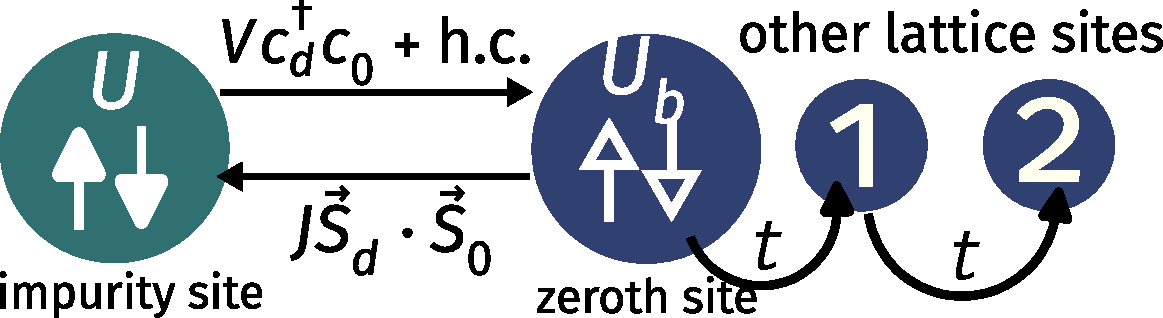
\includegraphics[width=0.5\textwidth]{zeromode_bare.pdf}
}
\end{frame}

\section{Renormalisation of Couplings}

\begin{frame}{Renormalisation of couplings}
Check how the Hamiltonian looks like at \alert{low energies}!
\vspace*{\fill}

\only<1>{
	1. Separate the Hamiltonian into a tower of energy scales

	\[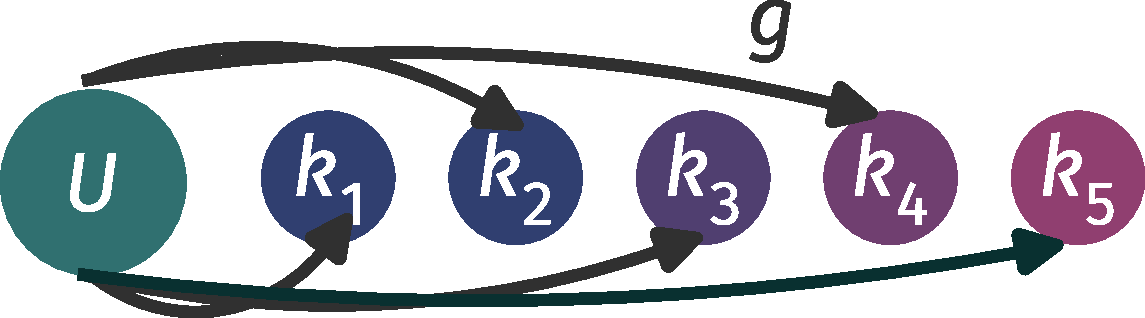
\includegraphics[width=0.5\textwidth]{siam_RG1.pdf}\]

	Kinetic energy of non-interacting problem provides an obvious scheme.
	\[\epsilon_0 > \epsilon_1 > \ldots > \epsilon_N \]
}
\only<2>{
	2. Integrate out the high energy degrees of freedom

	\[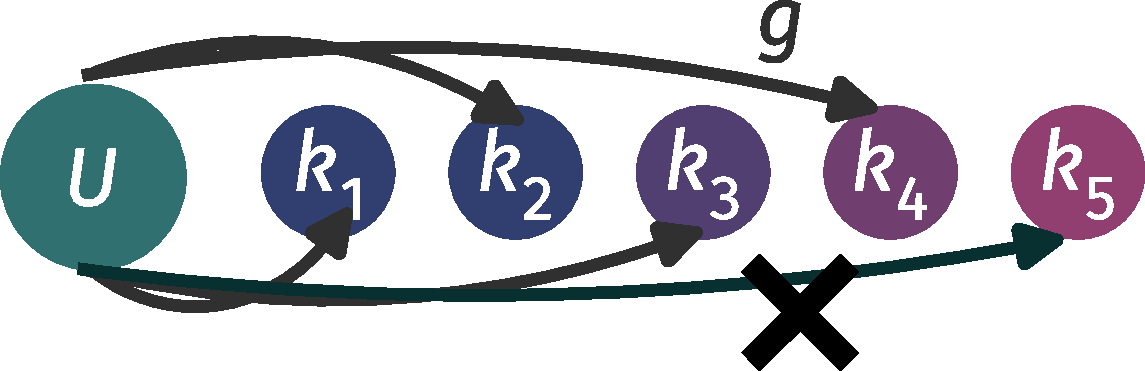
\includegraphics[width=0.5\textwidth]{siam_RG2.pdf}\]

	Involves removing number fluctuations in these states: 
	\[c^\dagger_\text{UV}, c_\text{UV} \to n_\text{UV}\]
}
\only<3>{
	3. Obtain renormalisation of remaining degrees of freedom

	\[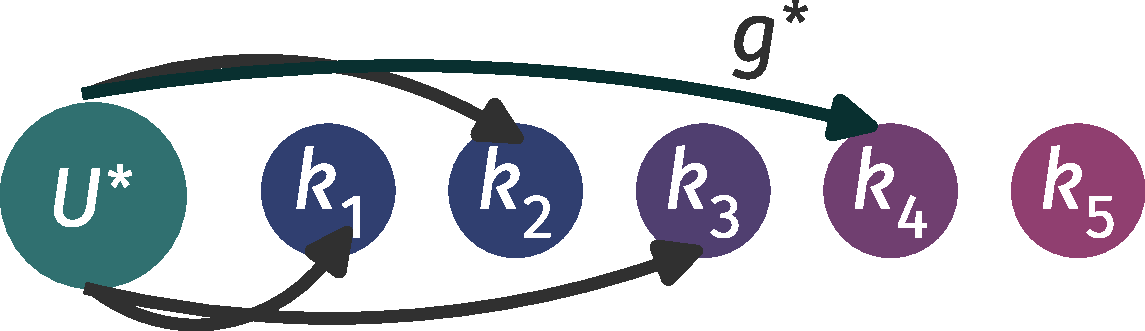
\includegraphics[width=0.5\textwidth]{siam_RG3.pdf}\]

	Virtual number fluctuations are taken into account: 
\[g^2 c^\dagger_{\text{UV}}c^\dagger_{\text{IR,1}} G_{\text{UV}} c_{\text{IR,2}}c_{\text{UV}} \sim g^* c^\dagger_{\text{IR,1}} c_{\text{IR,2}}\] 
}
\end{frame}

\begin{frame}{Renormalisation of couplings}
\eqbox{
\Delta J(D) = \frac{1}{\omega - D/2 + J/4}\rho(D) J\left( J + 4U_b \right)
}
Similar equations for \(V\) and \(U\); \alert{\(U_b\) is marginal}
\[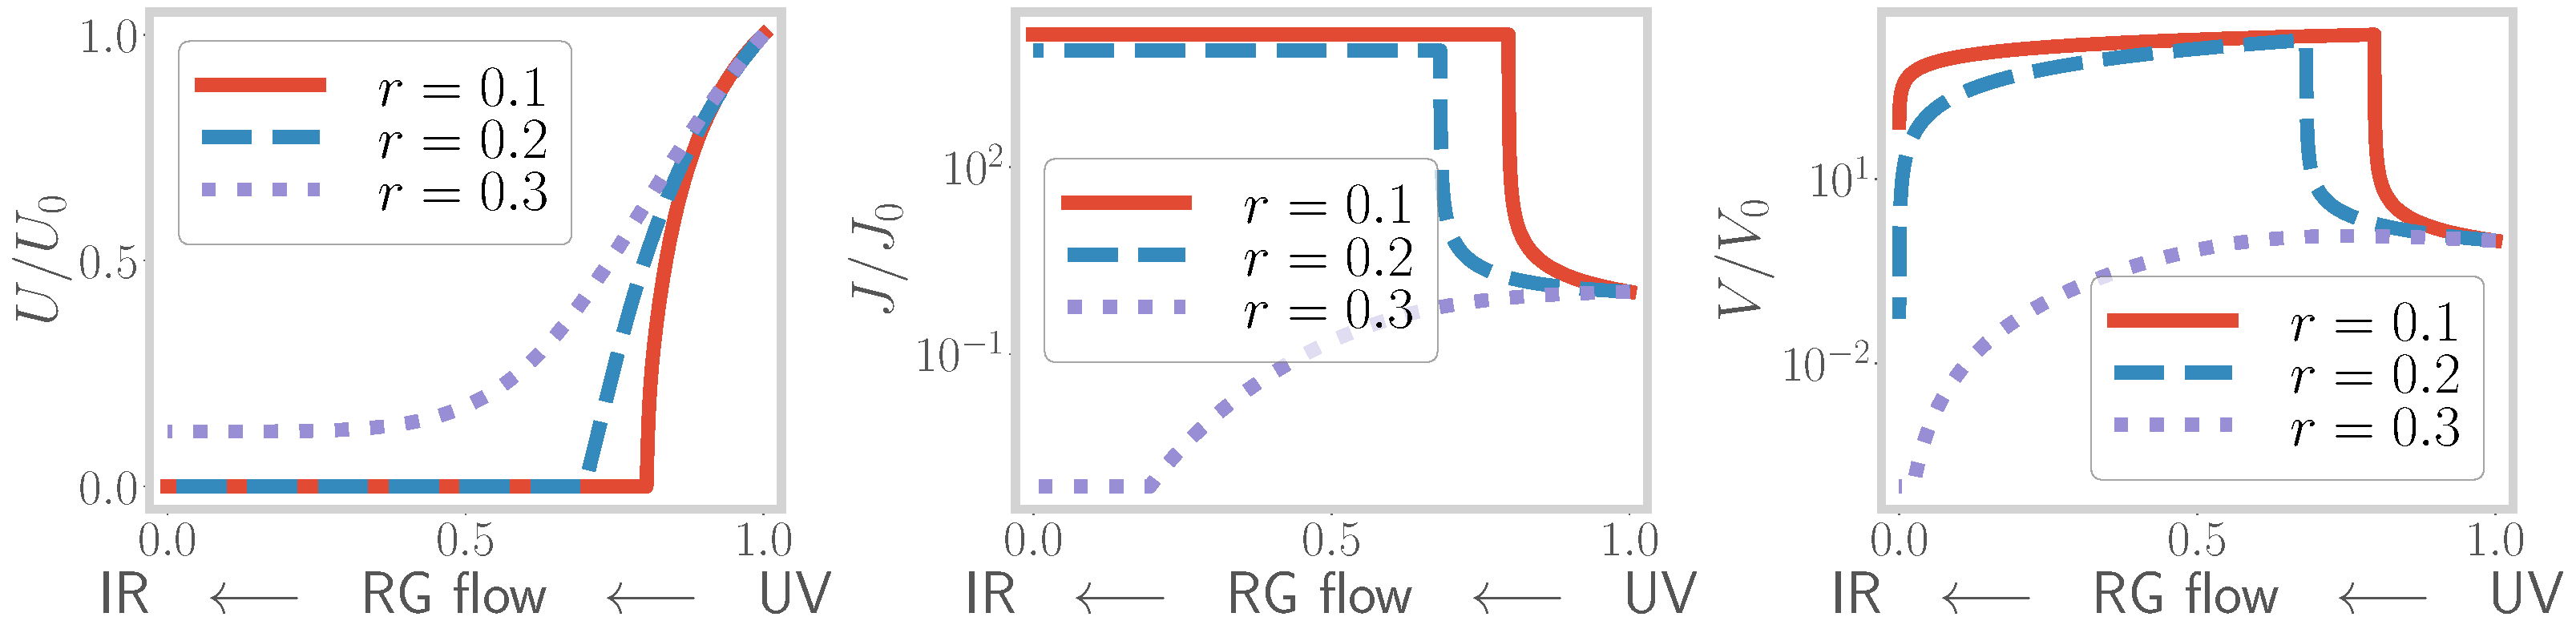
\includegraphics[width=\textwidth]{rg-flows-all.pdf}\]
\end{frame}

\begin{frame}{Renormalisation of couplings}
\alert{A closer look at the RG equation for J}

In terms of dimensionless couplings \(g = \rho\left( J + 2U_b \right) \) and \(\gamma = -2\rho U_b\):
\eqbox{
\Delta g \sim g^2 - \gamma^2\nonumber
}
\only<2->{
\vspace*{15pt}
\flushleft
\(U_b\) acts in two ways:
\begin{itemize}
	\item The first term represents an \alert{effective Kondo} RG flow with reduced strength \(g\)
	\item The second term is a \alert{new term that competes} with the effective Kondo effect
\end{itemize}
}
\only<3>{
\vspace*{15pt}
\flushleft
Kondo effect is \alert{destroyed} when the terms become of equal strength: 
\eqbox{
g = \gamma \implies r = -U_b/J = 0.25
}
}
\end{frame}

\section{\(T=0\) Phase Diagram}
\begin{frame}{Phase diagram}
\begin{minipage}{0.48\textwidth}
\vspace*{-14pt}
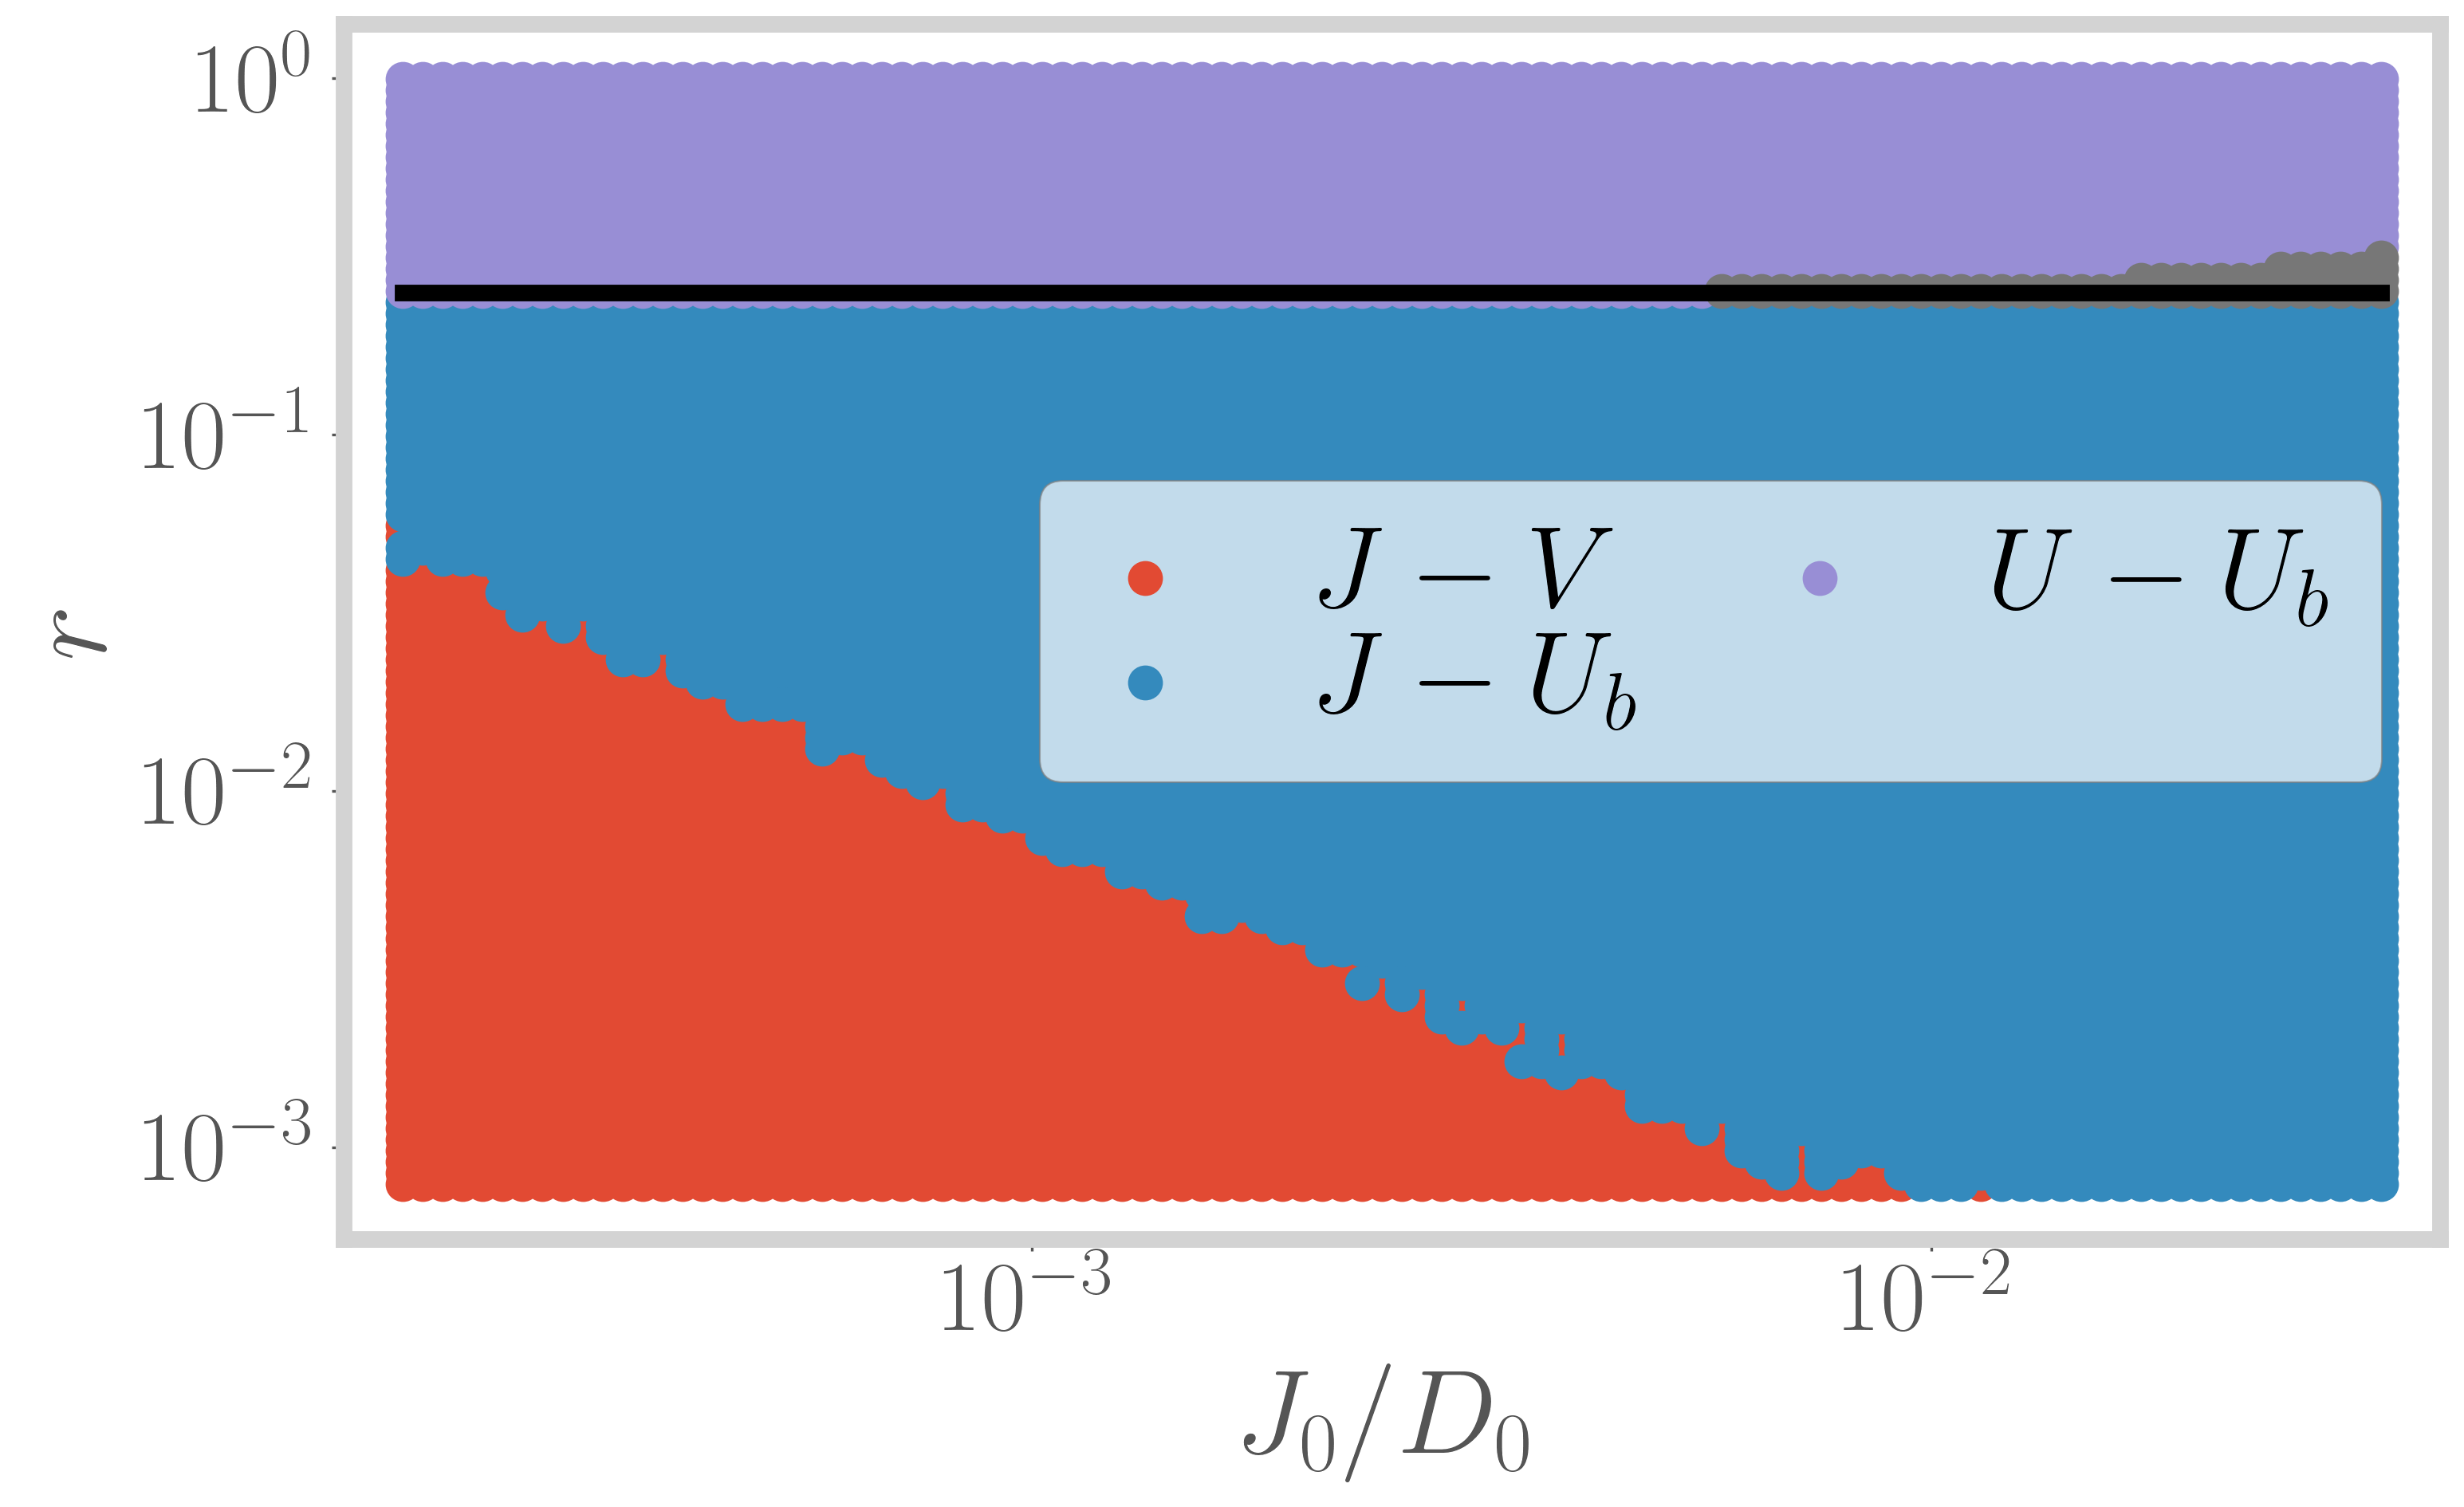
\includegraphics[width=\textwidth]{phase-map-MIT.png}
\end{minipage}
\begin{minipage}{0.48\textwidth}
\only<1>{
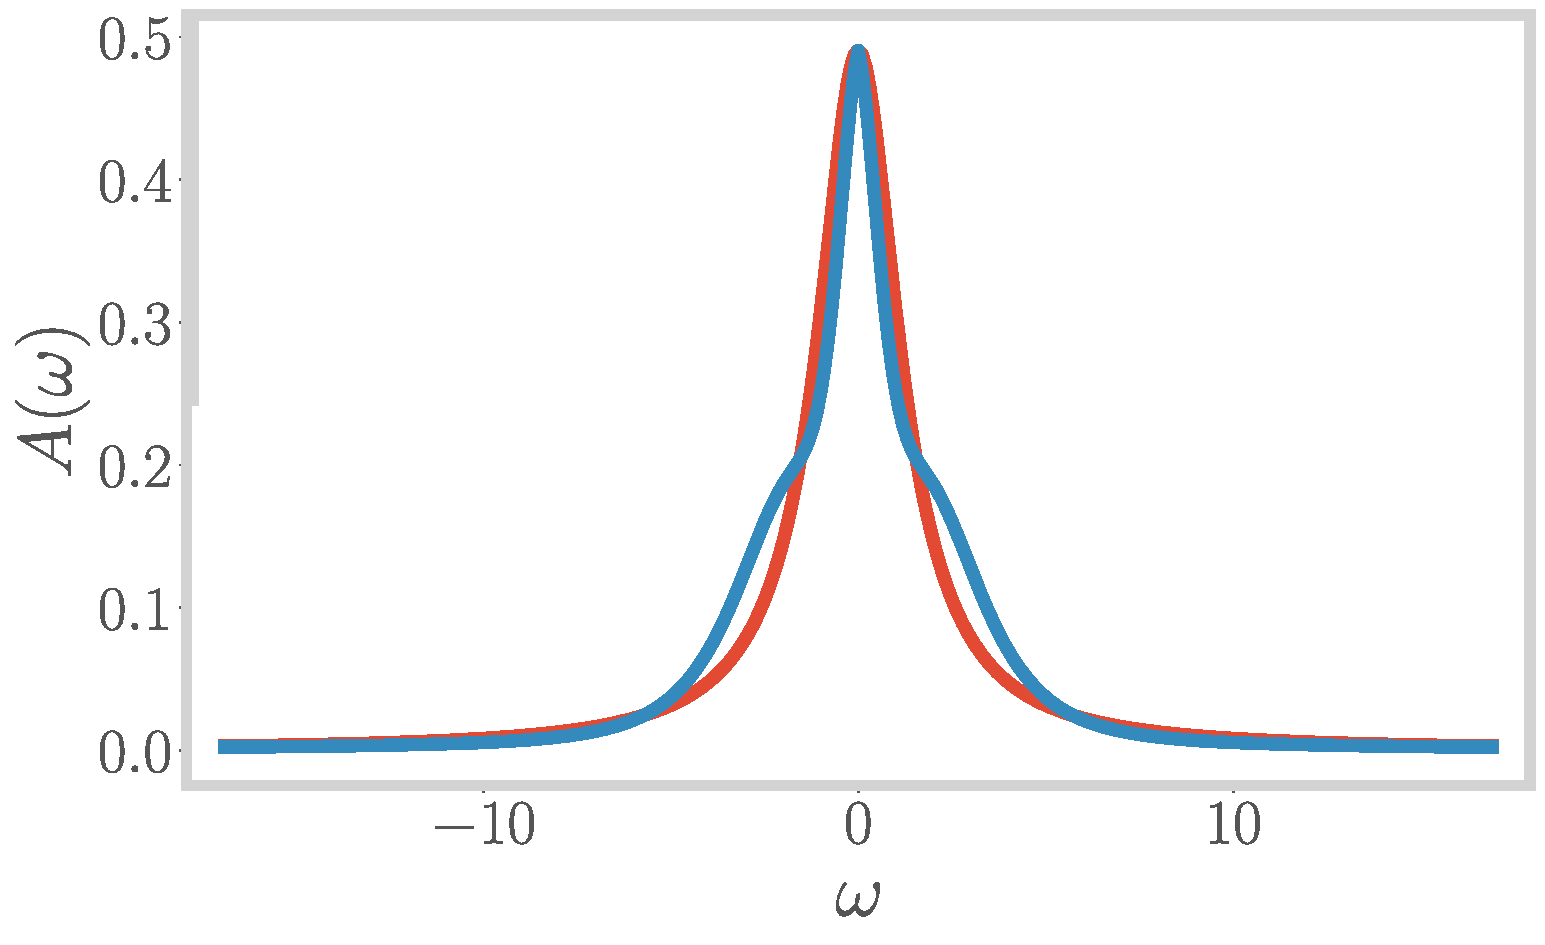
\includegraphics[width=\textwidth]{spectral-function1.pdf}
}
\only<2>{
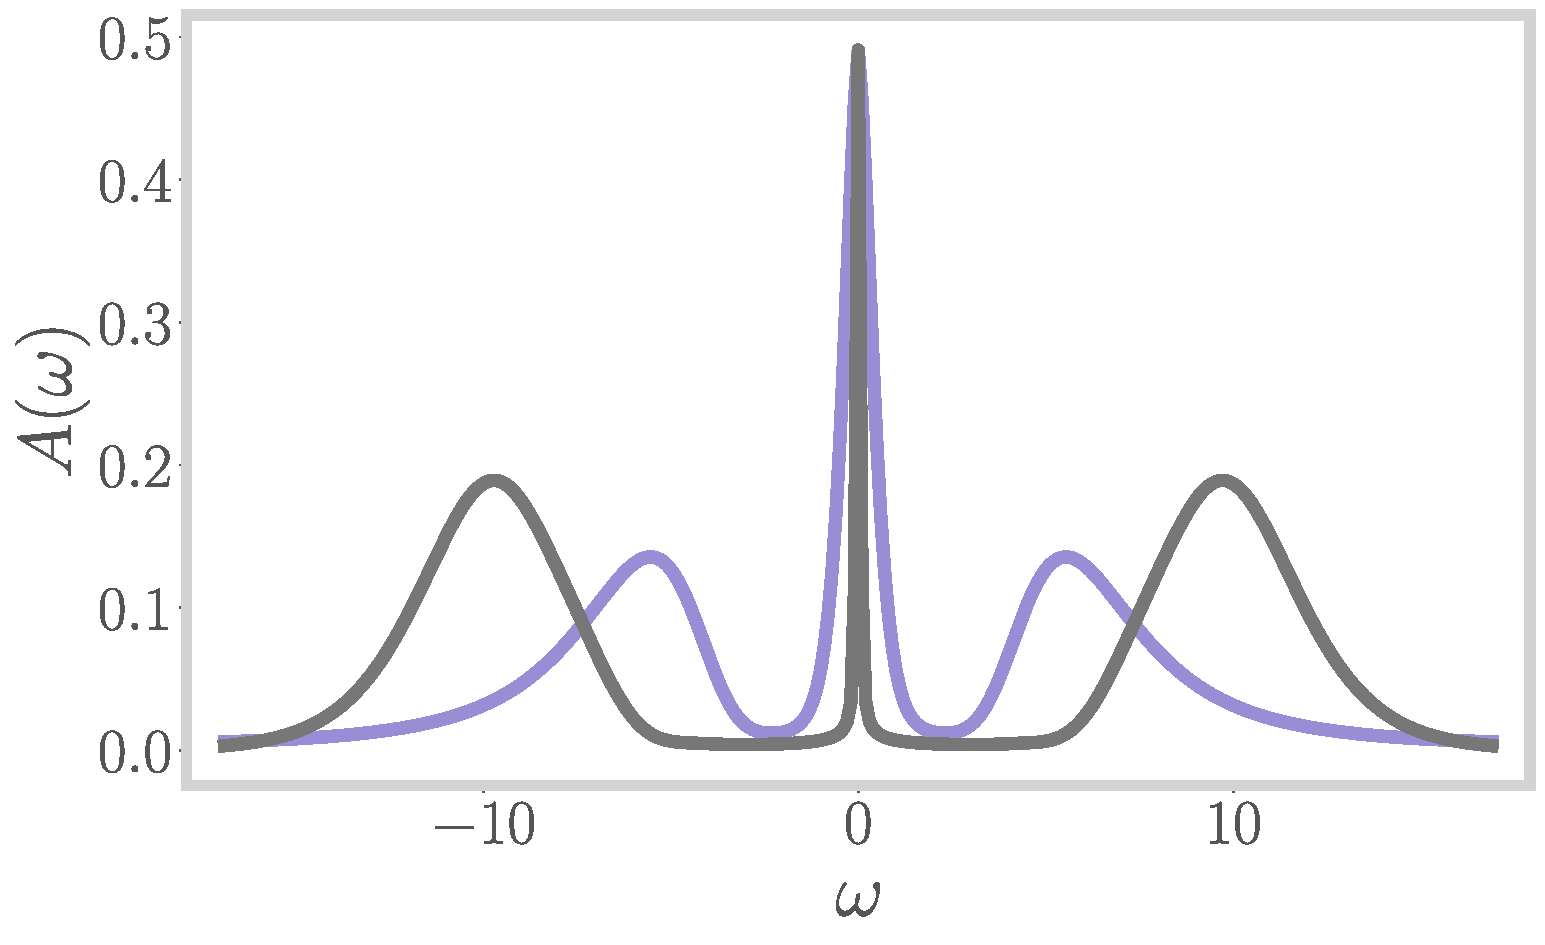
\includegraphics[width=\textwidth]{spectral-function2.pdf}
}
\only<3>{
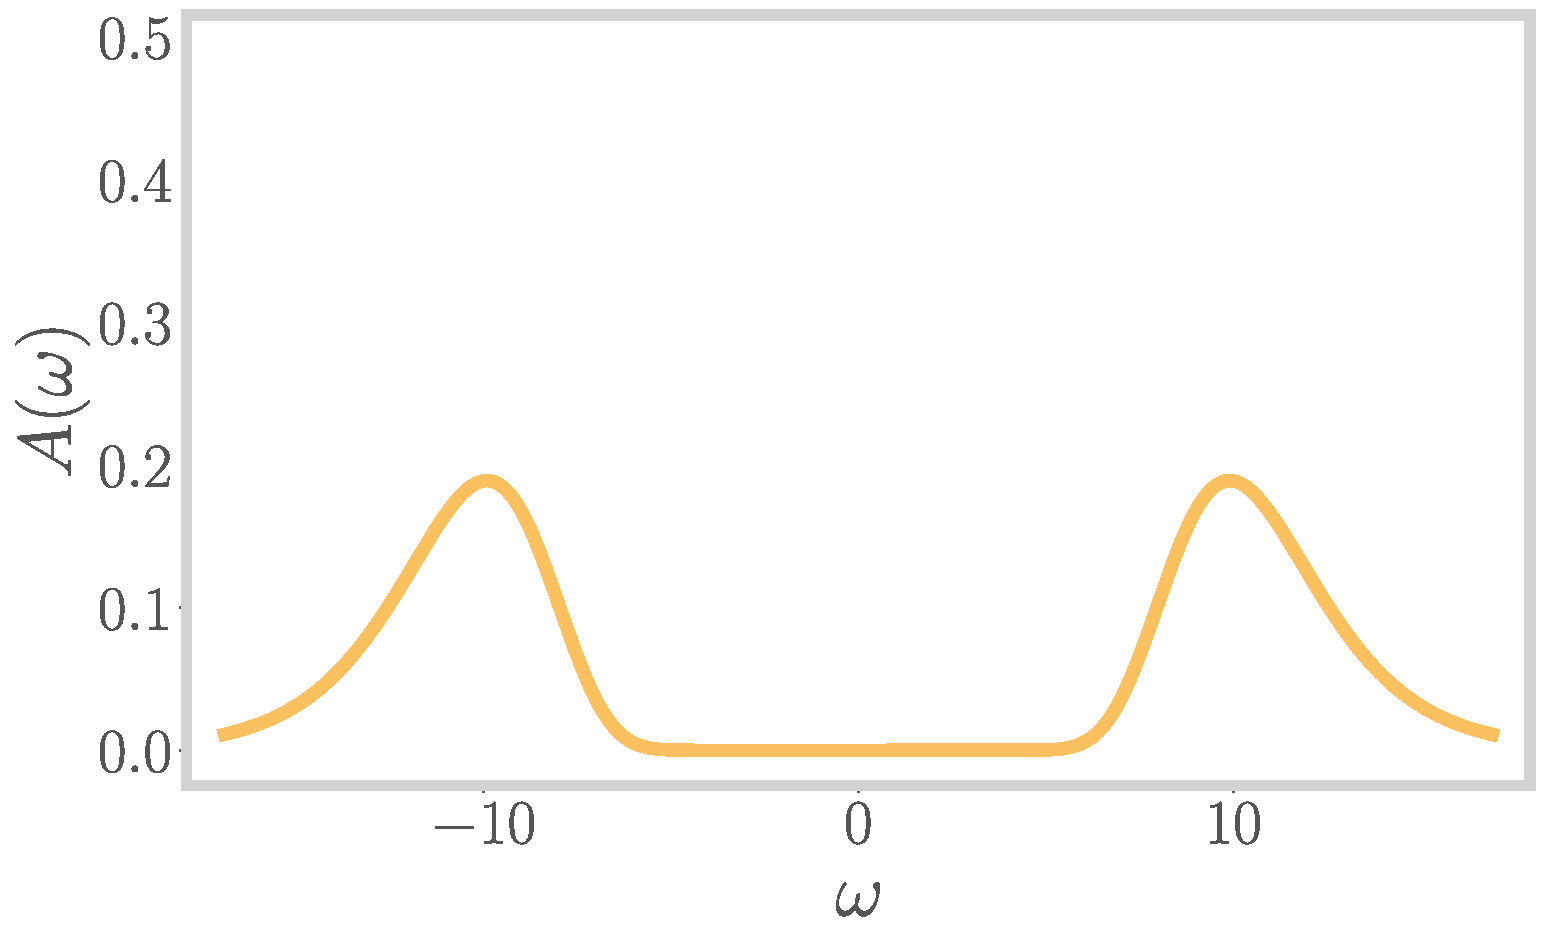
\includegraphics[width=\textwidth]{spectral-function3.pdf}
}
\end{minipage}
\only<1>{\alert{Red phase: weakly correlated metal}}
\only<2>{
\alert{Blue phase: strongly correlated metal}
}
\only<3>{
\alert{Violet phase: local moment}
}
\begin{minipage}{0.7\textwidth}
\begin{itemize}
\only<1>{
	\item \(V,J\) are relevant; broad spectral function\\[10pt]
	\item Effective Hamiltonian: \(H^*_\text{KE} + V^* \left( c^\dagger_{d\sigma}c_{0\sigma} + \text{h.c.} \right) + J^* \vec{S}_d\cdot\vec{S}_0\)\\[10pt]
	\item Ground state has both spin and charge content;
}
\only<2>{
	\item \(J\) relevant, \(V\) irrelevant; sharp spectral function\\[10pt]
	\item Effective Hamiltonian: \(H^*_\text{KE} + J^* \vec{S}_d\cdot\vec{S}_0 + \frac{U_b}{2}\left( n_{0 \uparrow} - n_{0 \downarrow} \right)^2 \)\\[10pt]
	\item Ground state has only spin - Kondo singlet;
}
\only<3>{
	\item \(V,J\) are irrelevant; gapped spectral function\\[10pt]
	\item Effective Hamiltonian: \(H^*_\text{KE} + \frac{U^*}{2}\left( n_{0 \uparrow} - n_{0 \downarrow} \right)^2 \)\\[10pt]
	\item Ground state reduces to a decoupled moment;
}
\end{itemize}
\end{minipage}
\begin{minipage}{0.29\textwidth}
\only<1>{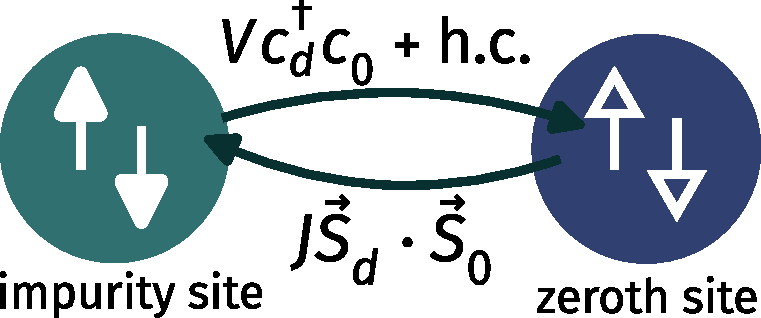
\includegraphics[width=\textwidth]{phase1.pdf}}
\only<2>{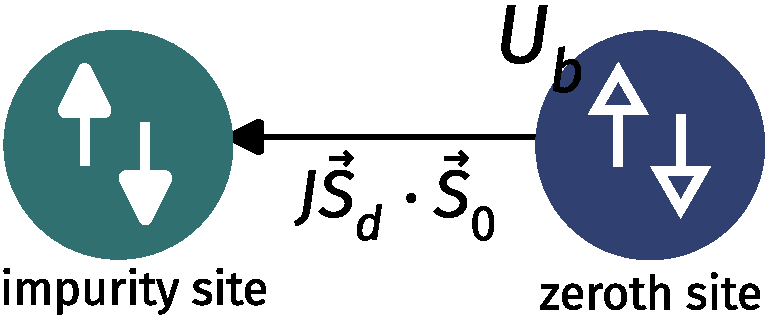
\includegraphics[width=\textwidth]{phase2.pdf}}
\only<3>{
\includegraphics[width=\textwidth]{phase3.pdf}}
\end{minipage}
\end{frame}

\begin{frame}[allowframebreaks]{References}
\printbibliography[heading=none]
\end{frame}

\end{document}
